\documentclass[11pt]{article}

% ------- Enable UTF8 characters ------- %
\usepackage[utf8]{inputenc}
\usepackage[english]{babel}

\usepackage[toc,page]{appendix}

\usepackage{listings}
\usepackage{color}
\usepackage[colorinlistoftodos]{todonotes}

\usepackage{epstopdf}
\usepackage{wrapfig}
\usepackage{pdfpages}
\usepackage{todonotes}
\usepackage{multicol}
\usepackage{amsmath}
\usepackage{amssymb}

% ------------ Code Listing ------------- %

\definecolor{dkgreen}{rgb}{0,0.6,0}
\definecolor{gray}{rgb}{0.5,0.5,0.5}
\definecolor{mauve}{rgb}{0.58,0,0.82}

\lstset{frame=false,
  language=VHDL,
  aboveskip=3mm,
  belowskip=3mm,
  showstringspaces=false,
  columns=flexible,
  basicstyle={\small\ttfamily},
  numbers=left,
  numberstyle=\tiny\color{gray},
  keywordstyle=\color{blue},
  commentstyle=\color{dkgreen},
  stringstyle=\color{mauve},
  breaklines=true,
  breakatwhitespace=true,
  tabsize=3,
  moredelim=**[is][\color{mauve}]{@}{@},
}

% ------- Page layout ------- %
\usepackage{fullpage}
\usepackage{hyperref} % clickable references
\hypersetup{
    colorlinks,
    citecolor=black,
    filecolor=black,
    linkcolor=black,
    urlcolor=black
}
\usepackage{multicol}
\setlength{\columnsep}{1cm}

% ------- Images ------- %
\usepackage{graphicx}
\usepackage{caption}
\usepackage{float}
%\usepackage{subfigure}
\usepackage{subcaption}
%\DeclareCaptionFont{gray}{\color{gray}}
%\captionsetup{textfont={footnotesize,sc,gray},font={footnotesize,sc,gray}}

\newcommand{\figscale}{0.7\linewidth}
\newcommand{\smallfigscale}{0.07\linewidth}

\usepackage{blindtext}



%References
\usepackage[numbers]{natbib} %Natbib supports both [i] and Author (year) citation styles. \citet and \citep replace \cite.
\bibliographystyle{ieeetr}
%\bibliographystyle{plainnat}
\usepackage{url}



% Test

\usepackage{tikz}
\usetikzlibrary{shapes,arrows,shadows}
\newcommand{\mx}[1]{\mathbf{\bm{#1}}} % Matrix command
\newcommand{\vc}[1]{\mathbf{\bm{#1}}} % Vector command

\begin{document}
\begin{titlepage}
\newcommand{\HRule}{\rule{\linewidth}{0.5mm}} % Defines a new command for the horizontal lines, change thickness here

\center % Center everything on the page
 
%----------------------------------------------------------------------------------------
%	HEADING SECTIONS
%----------------------------------------------------------------------------------------

\textsc{\LARGE University of Southern Denmark}\\[1cm] % Name of your university/college
\textsc{\Large SML-F16}\\[0.3cm] % Major heading such as course name
\textsc{\large Statistical Machine Learning }\\[0.3cm] % Minor heading such as course title
\vspace{0.5cm}
\begin{figure}[H]
\centering

\includegraphics[scale=1]{img/sdu-segl.png}
\end{figure}
\vspace{0.4cm}
%----------------------------------------------------------------------------------------
%	TITLE SECTION
%----------------------------------------------------------------------------------------

\HRule \\[0.4cm]
{ \huge \bfseries Applying k-Nearest Neighbours and Support Vector Machines to hand-written digit recognition}\\[0.4cm] % Title of your document
\HRule \\[2.5cm]
 
%----------------------------------------------------------------------------------------
%	AUTHOR SECTION
%----------------------------------------------------------------------------------------

\begin{minipage}{0.4\textwidth}
\begin{flushleft} \large
\emph{Authors:}\\
BSc. Mikael \textsc{Westermann}\\
\url{miwes12@student.sdu.dk}\\
BSc. Keerthikan \textsc{Ratnarajah}\\ % Your name 
\url{kerat12@student.sdu.dk}
\end{flushleft}
\end{minipage}
~
\begin{minipage}{0.4\textwidth}
\begin{flushright} \large
\emph{Supervisors:} \\
Prof. Norbert \textsc{Krüger}\\ % Supervisor's Name
ph.d. Troels Bo \textsc{Jørgensen}\\
\end{flushright}
\end{minipage}\\ %[3cm]

% If you don't want a supervisor, uncomment the two lines below and remove the section above
%\Large \emph{Author:}\\
%John \textsc{Smith}\\[3cm] % Your name

%----------------------------------------------------------------------------------------
%	DATE SECTION
%----------------------------------------------------------------------------------------
\vfill
{\large \today} %\\[3cm] % Date, change the \today to a set date if you want to be precise

%----------------------------------------------------------------------------------------
%	LOGO SECTION
%----------------------------------------------------------------------------------------

%\includegraphics{Logo}\\[1cm] % Include a department/university logo - this will require the graphicx package
 
%----------------------------------------------------------------------------------------

%\vfill % Fill the rest of the page with whitespace


\end{titlepage}
\tableofcontents
\newpage
\listoffigures
\listoftables
\newpage
\section{Introduction}
<<<<<<< HEAD
\todo[inline]{Something...}
The purpose of this report is to develop a system capable of recognizing hand writting characters such as digits (0 - 9).  This report will contain different approaches of classifying this, and their performance.  The dataset used for training and testing the performance of this, has be been made by the students of the statical machine learning class  as seen in \ref{fig:data}. The dataset consist of 400 $\times$ 10 individually handwritten numbers,  provided by each  student of the class.  

\begin{figure}[H]
\centering
\includegraphics[width =0.6\textwidth]{../../SML-database/2016/group2/member1/Ciphers100-0.png}
\caption{Example of the  dataset}
\label{fig:data}
\end{figure} 

The process of recognizing the digits can be divided into 3 steps. 
\begin{itemize}
\item Preprocessing - Extracting the data, and discard irrelevant information. 
\item Feature extraction - Extracting relevant features 
\item Classification - Use the extracted to classify the digits. 
\end{itemize}

=======
>>>>>>> 34ff1c3365fe38aae75203e9098a9fe6bb020ed5
 % Intro
%\chapter{kNN}
K - nearest - neighbor or kNN,
is a method for classifying objects based on the distance
to features extracted from ones training data.
The idea in kNN is to identiy k observation which is closest to the new
observation trying to be classified.
 The class with most vote determines which class the new observation
will be classified as. 
K is arbitrarily choosen by the user,
 and has an effect of the peformance of the algorithm. 
k-nn has an optimal classification rate when k becomes very large, 
but will computation wise take more time and vice versa. 
%\section{SVM}
Support vector machines is a supervised learning method that analyzes the data and tries to recognize patterns, within the classification domain. The standard SVM method is an binary classifier, which predicts for a given input which class the input belongs two. Prediction is done based on the model it builds from the training session, the model provides a "clear gap" that provide the distinction between the first or the latter class. \\

Support vector machine constructs a hyperplane or set of hyperplanes in a high dimension. The hyperplane that has the largest distance to the nearest training data points of any class (so-called functional margin), provides the best separation,  since it result it a clear distinction between the classes, and lower general error.
\\

The goal in SVM is to find this hyperplane which provides the optimal separation of the classes by having the widest margin. 

\begin{figure}[H]
\centering
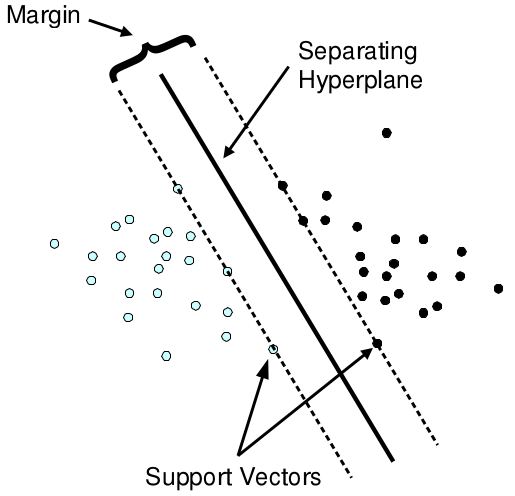
\includegraphics[width = 0.5\textwidth]{img/SVM-illu.png}
\caption{Svm Illustrated}
\label{fig::SVM-illustrated}
\end{figure}

The training data for this method consist a set of input vectors denoted as $\mathbf{x_i}$, each input vector has a number of component features. Each input vector is given a label, indicating its class.

The hyperplane is given as 
\begin{equation}
\mathbf{w} \cdot \mathbf{x} + b = 0
\end{equation}

In which the $\mathbf{w}$ determines the orientation of the plane, and $\mathbf{b}$ is the offset of the plane from the origin. \\
 
The seperaing hyperplane which maximizes the margin can be found by examining the convex hull of each class’s training data  and then find the closest points in the two convex hulls. The convex hull of a set of points is the
smallest convex set containing the points.  If the hyperplane that bisects both convex hulls can be found, will the resulting classifier deemed robust in some sense. 

\begin{figure}[H]
\centering
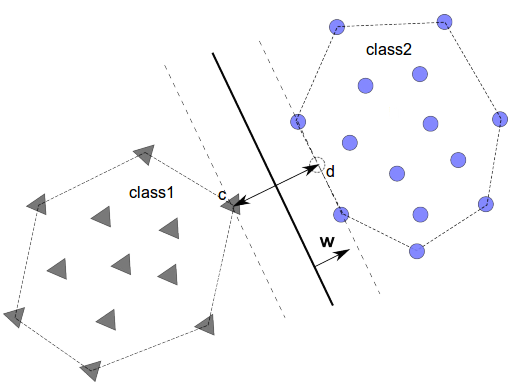
\includegraphics[width = 0.5\textwidth]{img/convex_hull.png}
\caption{best plane bisects closest points in the convex hulls,The convex hulls are labeled c and d}
\label{fig::convex_hull}
\end{figure}  

To find  the plane, one have to find the points closest to the plane, which can be found by solving the quadratic problem. \\ 

\begin{equation}
min_\alpha~\left(\frac{1}{2} ||c-d||^2\right)
\end{equation}

where c and d are the closest to be found points, these are defined as 
\begin{equation}
\begin{aligned}
&c = \sum_{y_i~\in~class1} \alpha_ix_i  
& \text{subject to}
&& \sum_{y_i~\in~class1}\alpha_i =1 
&& \alpha_i \geq 0
\end{aligned} 
\end{equation}

\begin{equation}
\begin{aligned}
&d = \sum_{y_i~\in~class2} \alpha_ix_i  
& \text{subject to}
&& \sum_{y_i~\in~class2}\alpha_i =1 
&& \alpha_i \geq 0
\end{aligned} 
\end{equation}


An alternative approach involves a search through the space of every possible hyperplane in order to find a set of two parallel planes that divide the points into homogeneous groups yet themselves are as far apart as possible.\\


In the case of non-linearly separable data, can a linear hyperplane not be used to define the solution. For this purpose is a slack variable introduced, which allows some points on the incorrect side of the margin, creating a soft margin, when a linear hyperplane was used to separate them.\\

A different approach for solving this problem would be using the kernel trick. The kernel trick involves transforming in $\mathbb{R}^n \rightarrow \mathbb{R}^{n+1}$. The challenging part is to find such transformation, $\phi$ which allow transforming data into a higher dimension. 

Kernel functions are in general in the following form:
\begin{equation}
K(\overrightarrow{x_i},\overrightarrow{x_j}) = \phi(\overrightarrow{x_i}) \cdot \phi(\overrightarrow{x_j}) 
\end{equation}

$x_i$ and $x_j$ illustrates two different feature vectors. 

Different kernels does already exist, and may already be implemented in different SVM software packages. 

\textbf{Linear kernel}:
\begin{equation}
K(\overrightarrow{x_i},\overrightarrow{x_j}) = (\overrightarrow{x_i}) \cdot (\overrightarrow{x_j}) 
\end{equation}

Linear kernel does not transform the data, but computes the dot product. 

\textbf{Polynomial kernel of degree $d$}:
\begin{equation}
K(\overrightarrow{x_i},\overrightarrow{x_j}) = ((\overrightarrow{x_i}) \cdot (\overrightarrow{x_j})+1)^d
\end{equation}

The Polynomial kernel adds a nonlinear transformation of the data.


\textbf{Sigmoid kernel}
\begin{equation}
K(\overrightarrow{x_i},\overrightarrow{x_j}) = tanh( k(\overrightarrow{x_i}) \cdot (\overrightarrow{x_j}) - \delta)
\end{equation}

The choice of kernel depends what kind of transformation is needed. 
%\chapter{PCA - Principal Component Analysis}
PCA is a tool used to find a low dimensional representation of a data set that represent as much variation as the complete data set.   The analysis finds uncorrelated variables named principal components from the dataset.  Using PCA would therefore also help lessen the change of "curse of dimensionality", and also improve the time needed to process the data. 

\begin{figure}[H]
\centering
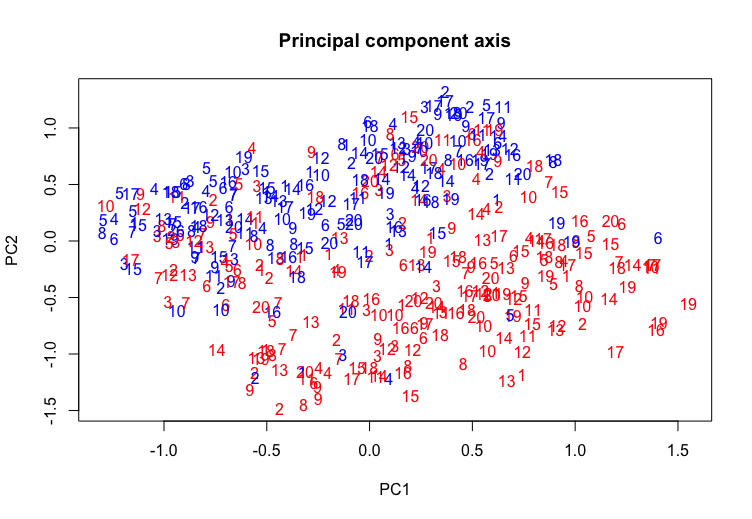
\includegraphics[width = \textwidth]{Figure/PCa-axis.png}
\caption{ red numbers indicated the axis of PC1 and the blue numbers determine the axis of PC2}
\label{fig:pca_vis}
\end{figure}

An illustration of the first two principal components of person dependent dataset can be seen in figure \ref{fig:pca_vis}. The axis shows how the data is distributed along both axis.  It shows that the PC1 axis has the greatest, as it can be seen from the variance of data aswell. 
\\
\\
As more PC gets included, will more of the variation of the dataset be exploited, and at the end completely resemble the the original data. The trick here is to find the right amount of PC which exploits the dataset as much as possible, and reduce the "unwanted" dimensions in the dataset. 

\begin{figure}[H]
\centering
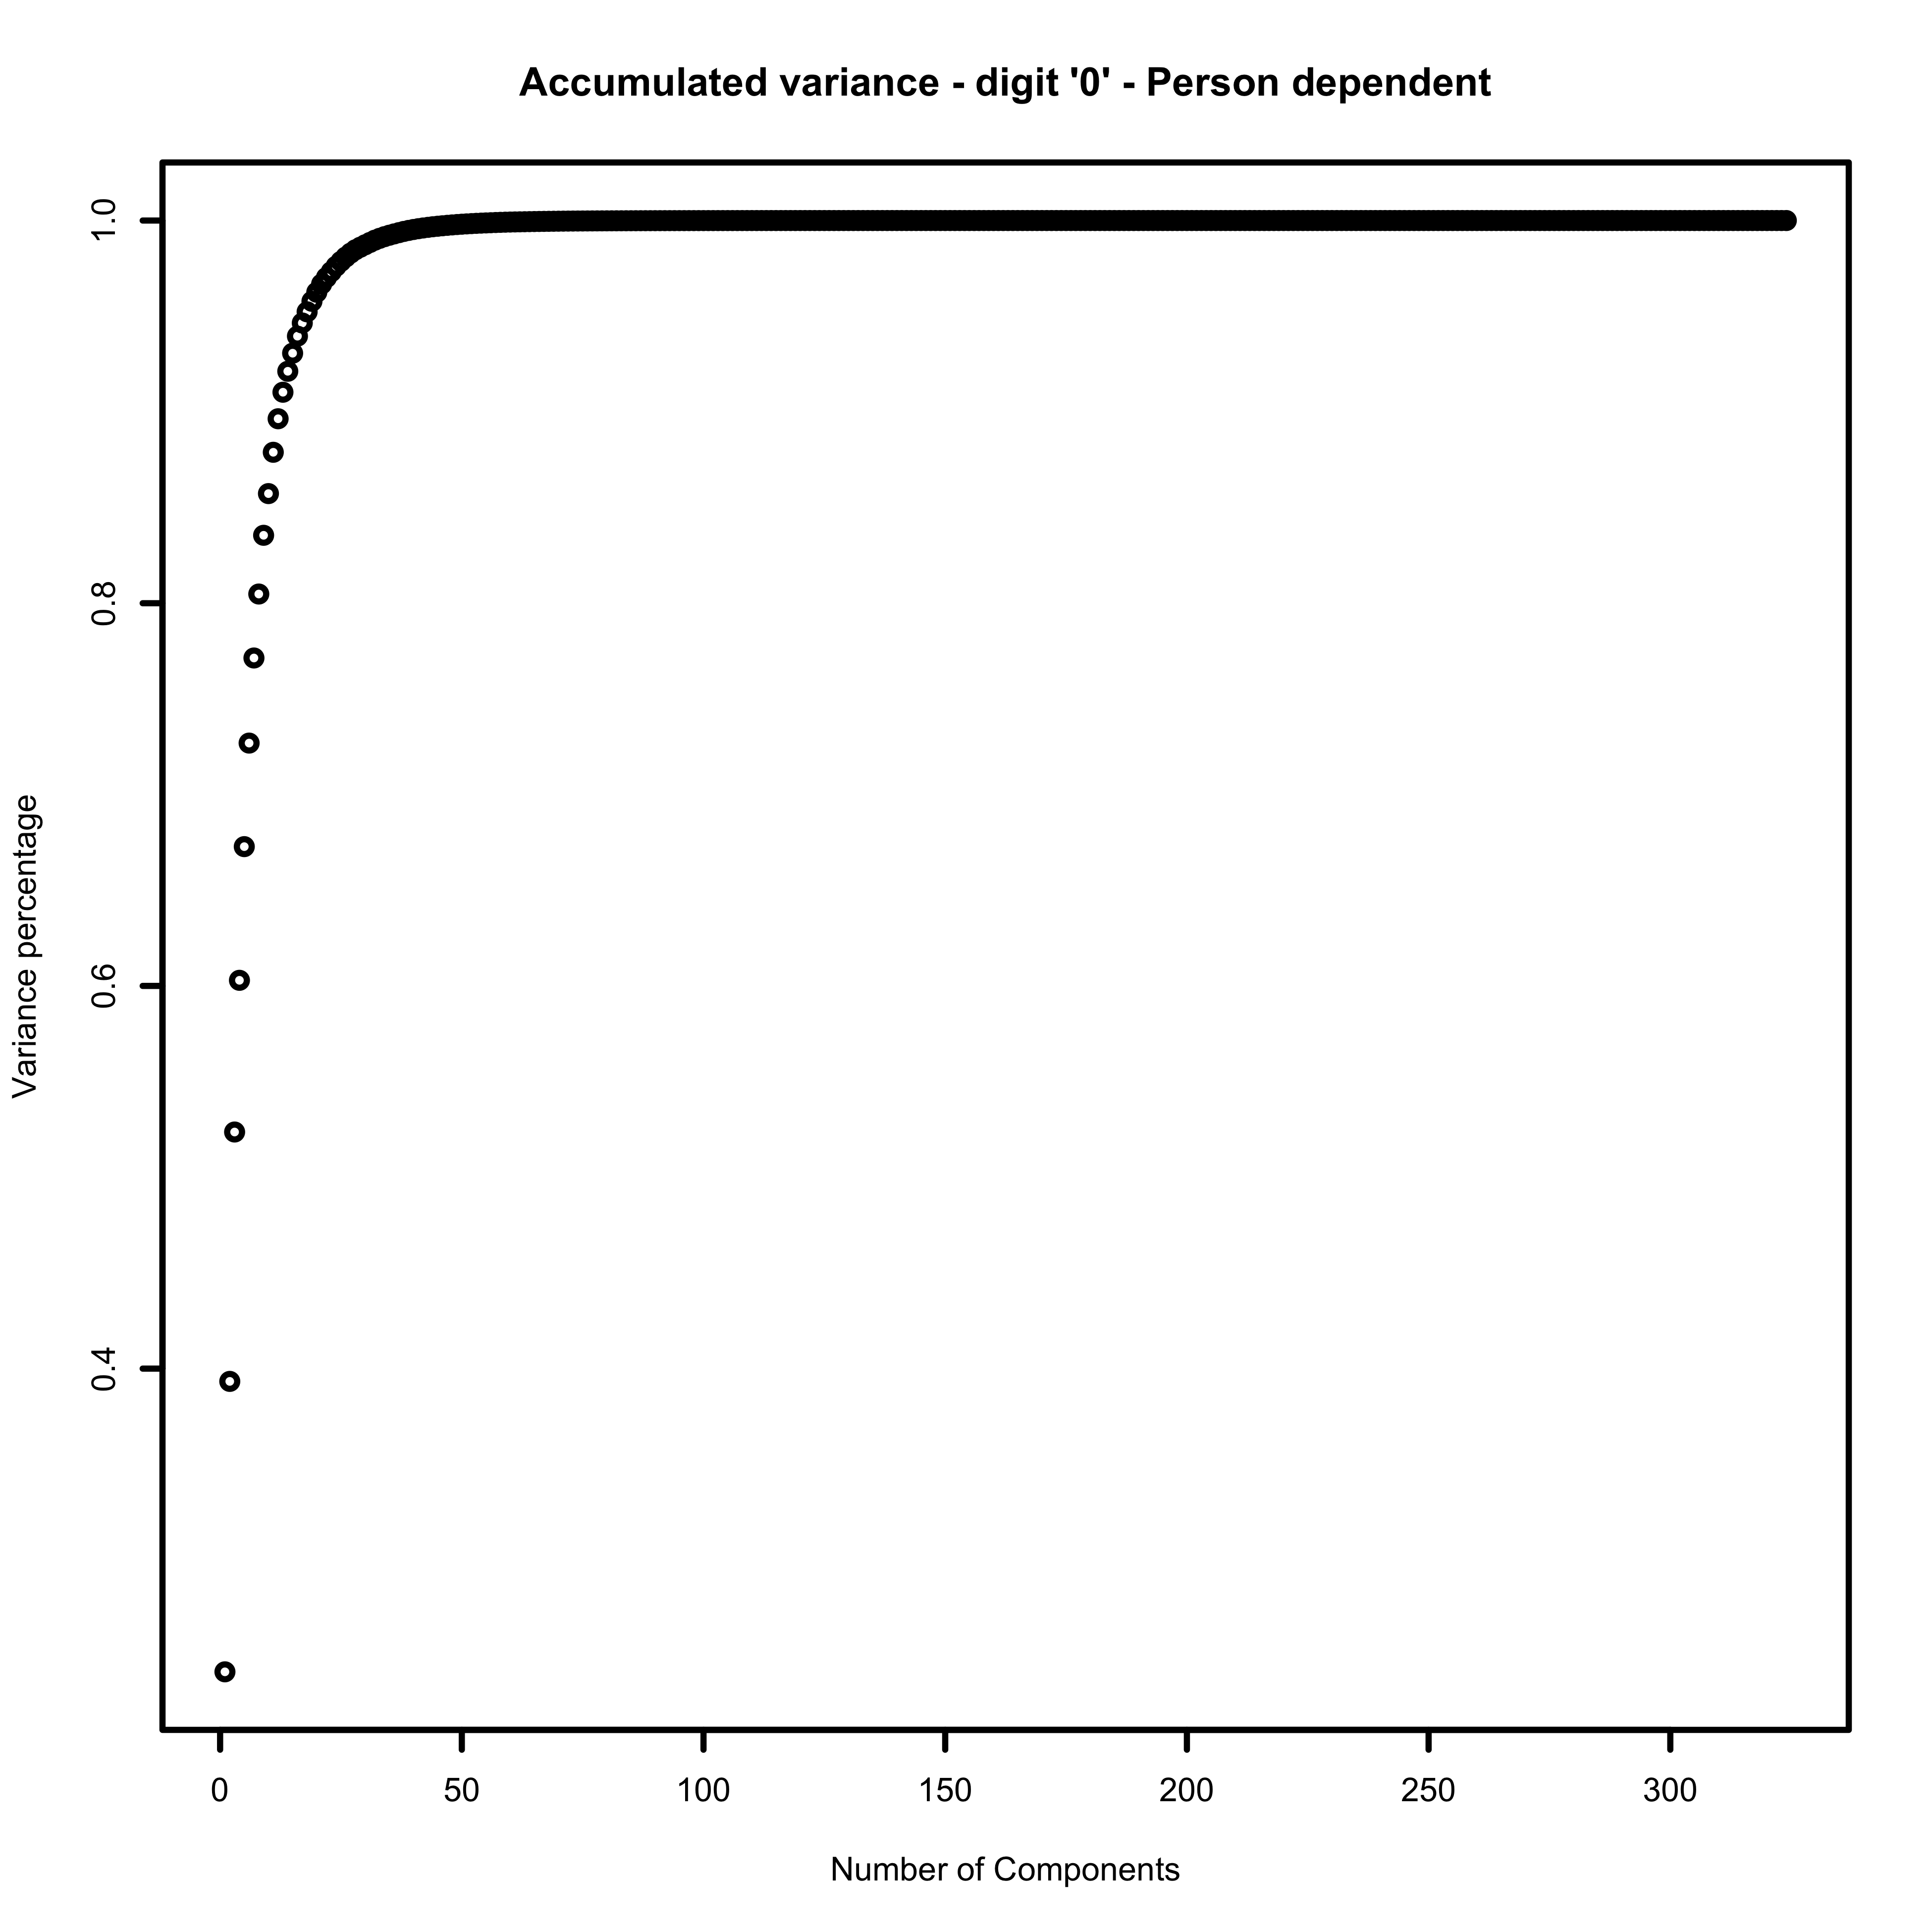
\includegraphics[width = 0.8\textwidth]{Figure/accumulated-2-1-person-dependent.png}
\caption{Plot showing the variance being accumulated for each component}
\label{fig:PCa_num_comp}
\end{figure}

As it can be seen in figure \ref{fig:PCa_num_comp} increased the accumalted variance strongly for the first principal components.  Using the elbow method one would be able to determine how many would be to determine how many would pc would fairly represent the dataset. 
\\
\\
\\
Using the PCA method were the dataset reduced into 4 sets  which represents 80\% , 90\%, 95\%, 99\% variances. The training was trained using a 10 - fold cross validation, which was repeated 10 times, and the accuracy mean was then computed. 

\begin{figure}[H]
\centering
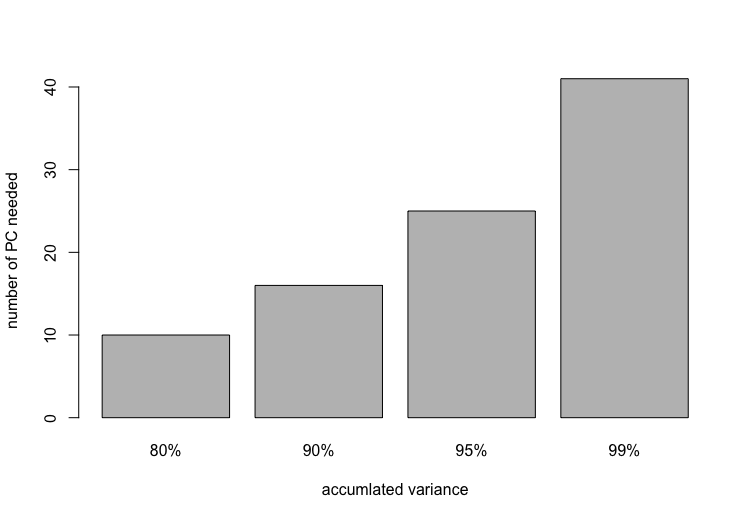
\includegraphics[width = \textwidth]{Figure/PCA_barplot.png}
\label{fig:pca_comp}
\caption{The number of components needed to achieve the desired variance}
\end{figure}

Using the PC were knn performed which resulted in this

\begin{figure}[H]
\centering
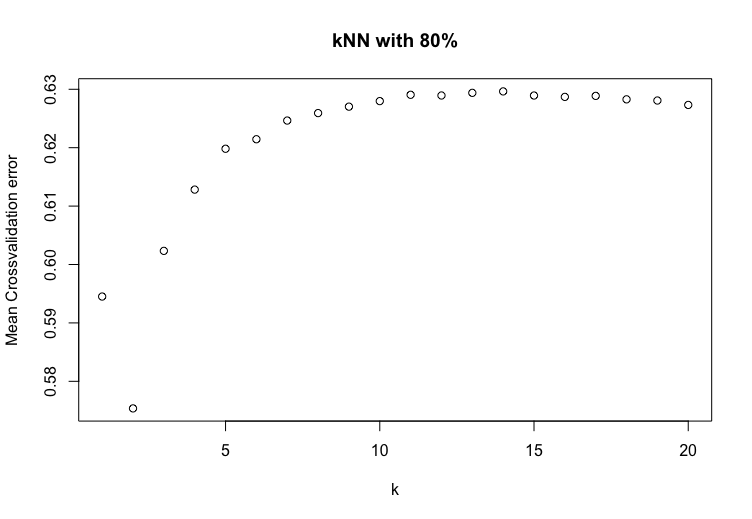
\includegraphics[width = \textwidth]{Figure/kNN_plot_80.png}
\label{fig:knnFit_80}
\end{figure}

\missingfigure{KnnFit Confusionmatrix}

\begin{figure}[H]
\centering
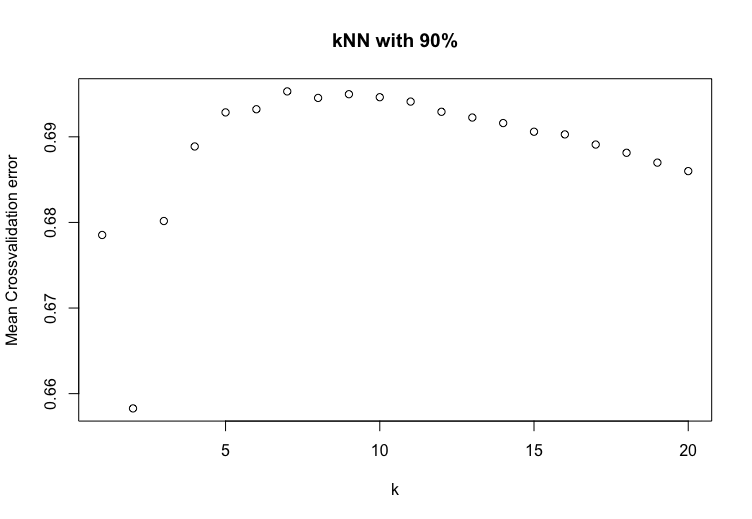
\includegraphics[width = \textwidth]{Figure/kNN_plot_90.png}
\label{fig:knnFit_90}
\end{figure}


\begin{figure}[H]
\centering
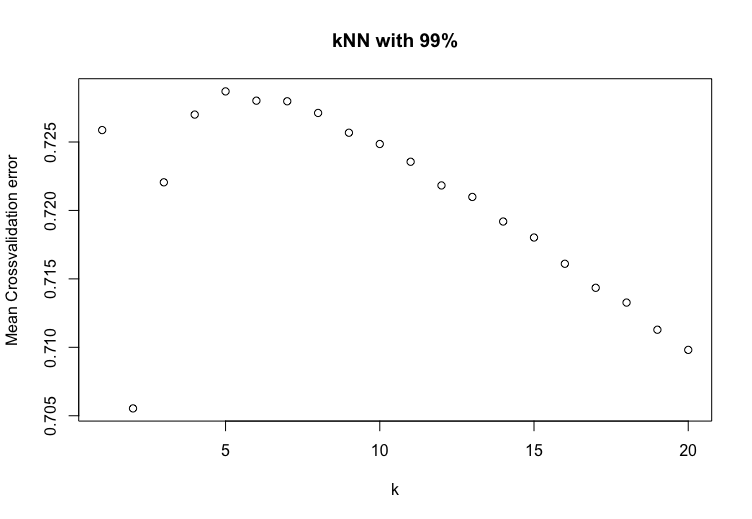
\includegraphics[width = \textwidth]{Figure/kNN_plot_99.png}
\label{fig:knnFit_99}
\end{figure}


\missingfigure{KnnFit plots}


\missingfigure{knnFit trainingTime}


\todo[inline]{prediction time.}
%\section{Preprocessing}
This section will entails details about the preprocessing step, what have been done to the scanned images, and why it has been done. 
\section{Methods}
\subsection{Preprocessing}
Each student of the 2016 class filled out several sheets of paper
with digits from 0 to 9. An example of this data
is shown in figure 
\ref{fig:handwriten_digits}. 
This section describes the preprocessing scheme
applied to this data before applying the machine learning algorithms.
\begin{figure}[h]
\centering
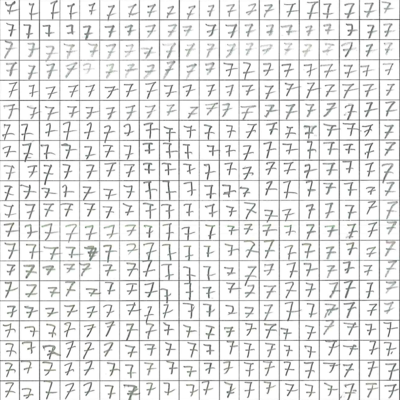
\includegraphics[width = 0.5\textwidth]{img/cropY2016G2M1-100-7.png}
\caption[Handwritten digits]
{
Handwritten digits. Scanned image. Cropped, rotated, scaled, stretched
and downsampled to 100 DPI.
}
\label{fig:handwriten_digits}
\end{figure}
Each of these sheets of paper was scanned by the student at a resolution of 300 DPI.

Each sheet held two 4x4" grids of 400 digits.
To ease the preprocessing task,
the student marked the pixel locations of the outer grid corners manually,
before submitting the dataset to the class database.

The datasets were of varying quality and format:
some images were color images while others were not,
most images were stretched and skewed to some degree,
and many digits were overlapping the grid.

As the corner locations were assumed to be known,
the images were rotated, stretched and scaled
by the perspective transform,
and then cropped,
to obtain ten images per student,
each being a 1200x1200 pixels image of 400 hand written digits.
This image was then downsampled to 200 DPI and to 100 DPI.
These preprocessing steps were done using MATLAB and ImageMagick.
After downsampling, the color images were converted to greyscale in R.

After color conversion, the images were smoothened in order
to make the digit data more uniform and easier to classify correctly.
It was chosen to apply a gaussian blur, as this smoothens
evenly in all directions.
The gaussian blur has one parameter named \(\sigma\),
and one which is the kernel size.
In this project, it was chosen to use the default
kernel size of \(2 \lceil3\sigma\rceil +1\),
and vary \(\sigma\) in order to find
optimal preprocessing parameters for the classification.

After smoothing the images of the grids,
each digit box (grid element) was extracted
as a vector of greyscale pixel intensities.
To avoid training the classifiers to recognize the parts
of the grid that are inside the digit boxes,
the digit boxes were cropped until the grid was no longer visible,
before vectorization.
A fixed cropping percentage of 10 \% along each border was used
(6 pixels border for 300 DPI, 4 pixels border for 200 DPI and 2 pixels border for 100 DPI).

Thus, at 300 DPI, a digit is represented in 2304 dimensions,
at 200 DPI, it is in 1024 dimensions,
and at 100 DPI, it is 256 dimensions.
Naturally, the computations involved in the classification
are faster when working with the lower-dimensional data.
As part of the \(\sigma\) optimization process,
it was therefore chosen to measure the k-NN classification
accuracy on the raw datasets at each pixel density,
giving an optimized \(\sigma\)-pixel density combination
for the digit recognition problem.

All above steps only need to be carried out once per
\(\sigma\)-pixel density combination.
The implemented R scripts thus compute this preprocessing
as an offline step, storing the preprocessed
datasets on disk.

\subsubsection{Principal Component Analysis}
In previous work, it was found that including Principal Component Analysis (PCA)
as a final step of the preprocessing could speed up the training
at an acceptable cost of reduced accuracy.

PCA is a statistical tool used for dimensionality reduction,
and works by creating new variables from the input variables.
These new variables, called principal components,
are linear combinations of the input variables,
and are ordered by how much of the input data variance they explain.
The statistical optimality of PCA is only achieved
when the input data is linear. This is not the case
for hand written digits. This may explain part
of the loss of accuracy.

As the main purpose of this project is the comparison of two algorithms,
it was chosen to apply PCA to the data before machine learning.
In addition, the PCA was used to verify the previous
steps of the preprocessing scheme qualitatively,
ensuring that the main data variance is not due to the grid lines of the input data.

The dimensionality reduction lies in transforming the input
data by a matrix representing the principal components
(the eigenvectors), and then using only the
first N components, enough to explain a given percentage of the cumulated variance.

The data transformation matrix obtained from one PCA
can be stored and applied to new data.
It was therefore chosen to include the PCA in the training of the classifiers,
storing the information necessary to transform new data
with the trained classifiers.
PCA is performed before training, on the training set,
and the number of components is chosen dynamically as the minimum
required to explain a given percentage of the cumulated variance
of the training set.
Thus, the tuning parameter investigated in this work,
is the percentage of the cumulated variance to explain,
making the PCA an online step of the preprocessing scheme.
The results of PCA are therefore not stored on disk,
except when saved along with trained classifiers.

\subsection{k-Nearest Neighbours}
k-Nearest Neighbours (k-NN)
is a supervised learning algorithm.
The method is non-parametric,
meaning that it does not make any assumption about the distribution of the input data.
The method is referred to as a lazy learning algorithm,
as it does not use the training data to do any generalization (abstraction).
Figure \ref{fig:knn-example} \citep{knnwiki} shows the basic principle of the algorithm.
\begin{figure}[h]
\centering
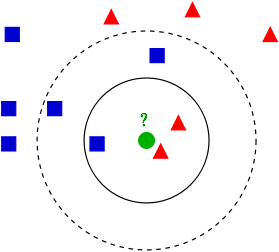
\includegraphics[width = 0.3\textwidth]{img/kNN-classification.png}
\caption[k-NN classification example]{
k-NN classification example, 2-dimensional 2-class data.
The test sample, the green circle,
has to be classified as one of the two classes indicated
as red triangles and blue squares, based on the number
of training samples close to the test samples.
With k=3 (the inner circle), the sample would be classified as belonging
to the class of the red triangles.
With k=5 (the outer dashed circle), the sample would be classified as belonging
to the class of the blue squares.
Author: Antti Ajanki \citep{knnwiki}.
}
\label{fig:knn-example}
\end{figure}

The purpose of the algorithm is to classify a
new \(n\)-dimensional test sample based on its \(n\) attributes
and the training samples that have been used.
The algorithm decides which class a new sample belongs to by
inspecting the k nearest neighbours,
and based on the class which is represented most strongly in the vicinity
of the test sample,
the class of the new sample is determined.
k can be both an even or an odd number.
In the case of a tie with a even numbered k,
the class of the test sample is randomly chosen among the classes holding
the majority of the votes.

The k-NN classifier performs differently with different k,
meaning k is a tuning parameter which can be used to optimize the classifier
to certain data.

Several metrics for measuring the distance between
two samples \(\mathbf{w}\) and \(\mathbf{v}\) can be employed,
including Euclidean distance, eq. \eqref{eq:euclidean-distance},
and Manhattan distance, eq. \eqref{eq:manhattan-distance}.
\begin{equation}
d(\mathbf{w},\mathbf{v}) = \sqrt{\sum_{i=1}^n (w_i - v_i)^2}
\label{eq:euclidean-distance}
\end{equation}
\begin{equation}
d(\mathbf{w},\mathbf{v}) = \sum_{i=1}^n \left|w_i - v_i\right|
\label{eq:manhattan-distance}
\end{equation}

The advantage of using k-NN is that it is simple to use,
and works well on basic problems.
However, it can be slow for real-time prediction applications,
especially if the dataset used for training is large,
as the method is a lazy learner.
Another disadvantage of the method is that it does not
learn anything from the training data, but just stores it;
No particular new insight is gained.
 
\subsection{Support Vector Machines}
Support Vector Machines (SVM) is a supervised learning
method that analyzes training data 
and tries to recognize patterns within the classification domain.
The standard SVM method is a binary classifier,
which predicts which of the two classes a given input belongs two. 
Prediction is done based on the model built from the training session.
The model provides a constraining border which makes the distinction
between the two classes.

For \(n\)-dimensional data,
SVM constructs an \(n\)-dimensional hyperplane or a set of hyperplanes.
The hyperplane with the largest distance to the nearest training sample
of any class (so-called functional margin), provides the best separation,
since it results in the clearest distinction between the classes,
and lower general error,
as illustrated by figure \ref{fig::SVM-illustrated} \citep{svmwiki}.

The goal in SVM is to find this hyperplane which provides the optimal separation 
of the classes by having the widest margin. 

\begin{figure}[h]
\centering
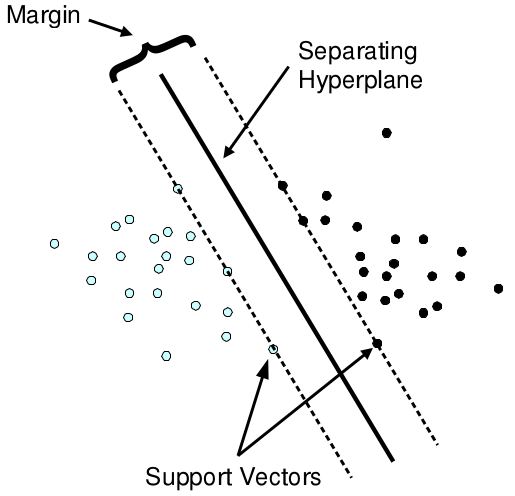
\includegraphics[width = 0.5\textwidth]{img/SVM-illu.png}
\caption[SVM Illustrated]{SVM Illustrated. Author: \citep{svmwiki}.}
\label{fig::SVM-illustrated}
\end{figure}

The training data for this method consist a set of input vectors denoted as 
$\mathbf{x_i}$, each input vector has a number of component features. Each input 
vector is given a label, indicating its class.

The hyperplane is given as 
\begin{equation}
\mathbf{w} \cdot \mathbf{x} + b = 0
\end{equation}

In which the $\mathbf{w}$ determines the orientation of the plane, and 
$\mathbf{b}$ is the offset of the plane from the origin. \\
 
The seperaing hyperplane which maximizes the margin can be found by examining 
the convex hull of each class’s training data  and then find the closest points 
in the two convex hulls. The convex hull of a set of points is the
smallest convex set containing the points.  If the hyperplane that bisects both 
convex hulls can be found, will the resulting classifier deemed robust in some 
sense. 

\begin{figure}[H]
\centering
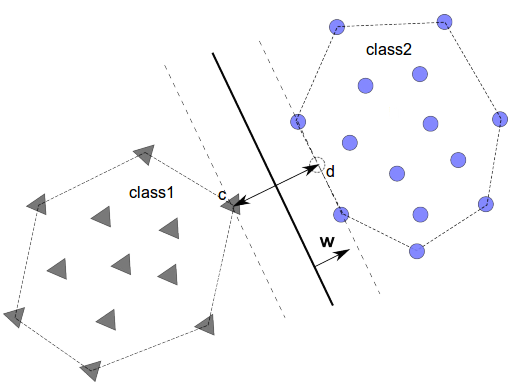
\includegraphics[width = 0.5\textwidth]{img/convex_hull.png}
\caption{Best plane bisects closest points in the convex hulls,The convex hulls 
are labeled c and d}
\label{fig::convex_hull}
\end{figure}  

To find  the plane, one have to find the points closest to the plane, which can 
be found by solving the quadratic problem. \\ 

\begin{equation}
min_\alpha~\left(\frac{1}{2} ||c-d||^2\right)
\end{equation}

where c and d are the closest to be found points, these are defined as 
\begin{equation}
\begin{aligned}
&c = \sum_{y_i~\in~class1} \alpha_ix_i  
& \text{subject to}
&& \sum_{y_i~\in~class1}\alpha_i =1 
&& \alpha_i \geq 0
\end{aligned} 
\end{equation}

\begin{equation}
\begin{aligned}
&d = \sum_{y_i~\in~class2} \alpha_ix_i  
& \text{subject to}
&& \sum_{y_i~\in~class2}\alpha_i =1 
&& \alpha_i \geq 0
\end{aligned} 
\end{equation}


An alternative approach involves a search through the space of every possible 
hyperplane in order to find a set of two parallel planes that divide the points 
into homogeneous groups yet themselves are as far apart as possible.\\


In the case of non-linearly separable data, can a linear hyperplane not be used 
to define the solution. 
For this purpose is a slack variable introduced, which allows some points on the 
incorrect side of the margin, creating a soft margin, when a linear hyperplane 
was used to separate them.\\

A different approach for solving this problem would be using the kernel trick. 
The kernel trick involves transforming in $\mathbb{R}^n \rightarrow 
\mathbb{R}^{n+1}$. 
The challenging part is to find such transformation, $\phi$ which allow 
transforming data into a higher dimension. 

Kernel functions are in general in the following form:
\begin{equation}
K(\overrightarrow{x_i},\overrightarrow{x_j}) = \phi(\overrightarrow{x_i}) \cdot 
\phi(\overrightarrow{x_j}) 
\end{equation}

$x_i$ and $x_j$ illustrates two different feature vectors. 

Different kernels does already exist, and may already be implemented in 
different SVM software packages. 
\\

\textbf{Linear kernel}:
\begin{equation}
K(\overrightarrow{x_i},\overrightarrow{x_j}) = (\overrightarrow{x_i}) \cdot 
(\overrightarrow{x_j}) 
\end{equation}

Linear kernel does not transform the data, but computes the dot product. 
\\

\textbf{Polynomial kernel of degree $d$}:
\begin{equation}
K(\overrightarrow{x_i},\overrightarrow{x_j}) = ((\overrightarrow{x_i}) \cdot 
(\overrightarrow{x_j})+1)^d
\end{equation}

The Polynomial kernel adds a nonlinear transformation of the data.
\\

\textbf{Sigmoid kernel}
\begin{equation}
K(\overrightarrow{x_i},\overrightarrow{x_j}) = tanh( k(\overrightarrow{x_i}) 
\cdot (\overrightarrow{x_j}) - \delta)
\end{equation}
\\

\textbf{Radial basis function kernel}
\begin{equation}
K(\overrightarrow{x_i},\overrightarrow{x_j}) =  
exp\left(\frac{||\overrightarrow{x_i} - 
\overrightarrow{x_j}||}{2\sigma^2}\right)
\end{equation}

In which the value $\gamma = \frac{1}{2\sigma^2}$ can be adjusted.\\


The choice of kernel depends what kind of transformation is needed. 

\subsection{Parameter optimization}
The k-NN and SVM classifiers were each trained on the \(D_{FEWER}\) dataset with the \textbf{LOO} method.

\subsection{Parameter optimization on a smaller dataset}
To extract the most optimal parameter for training purposes was it decided, optimize the parameter on a smaller set consisting of 10 people data.  This was choosen, as it was desired gain the most optimal values for the varied dataset, such that the parameter found would be fit for a specific scenario, but a broad case. 
\todo[inline]{might have to be adjusted..}

\subsection{Test with data from single person}
\label{sec::test_with_data_from_single_person}

The first training were conducted with every single persons training set. The 
training using kNN consisted of k = 5,with a 10 - fold cross validation. k = 5 
was chosen, as it was shown from the parameter optimization that it would provide the highest accuracy on a varied dataset. \\

The training using SVM were performed using a polynomial kernel, with a degree 
of 2, scale of 0.1   and cost of 0.5 with a 10 fold cross validation as well. 
The polynomial kernel was chosen due to prior experiments with other kernel, and 
had a higher degree of freedom would provide a better accuracy. The parameter chosen was also found from the parameter optimization section. 
\todo[inline]{maybe a bit fluffy idk?}

 
A
10-fold cross validation uses 1 fold for testing and the rest for training 
purposes it thereby provides an average of the accuracies on how well a trained 
classifier, trained using the persons own data is capable of detecting himself.  
This information provides some insight on how consistent the persons writing is. 
An inconsistent writing style will cause lower mean accuracy compared to a 
consistent style. \\

Each accuracy is given an error bar stating the standard deviation of the 
dataset. The standard deviation of the mean accuracy is found by adding the 
internal standard deviation and the external standard deviation. The internal 
standard deviation is a vector of all individual standard deviation acquired 
from the 10-fold cross validation, an the external consist of the variance 
between the accuracies acquired  from the 10-fold cross validation. \\
 
The result of this test can be seen in section  \ref{sec::result}. 

\subsection{Test with data from all persons with a training set that includes 
data from all}

The dataset used for training here consist all the data mixed together. A 10-fold crossfold validation was also applied on to it from which an accuracy was computed. 



\subsection{Test with data from all persons where the training set does not 
include data from 
the persons in the test set}

The dataset consist of all the person, where the test was performed by leaving one out. A 10-fold crossfold validation was also applied onto it from which an accuracy was computed. 





 %Metod
\section{Results}
\subsection{Downsampling}
With data from G2M2, k-NN prediction running times
were measured vs. dataset size N at various DPI.
The results
are presented in figure \ref{fig:knn-runningtime-vs-n-and-k}.
\begin{figure}[h]
	\centering
	\begin{subfigure}{0.32\textwidth}
		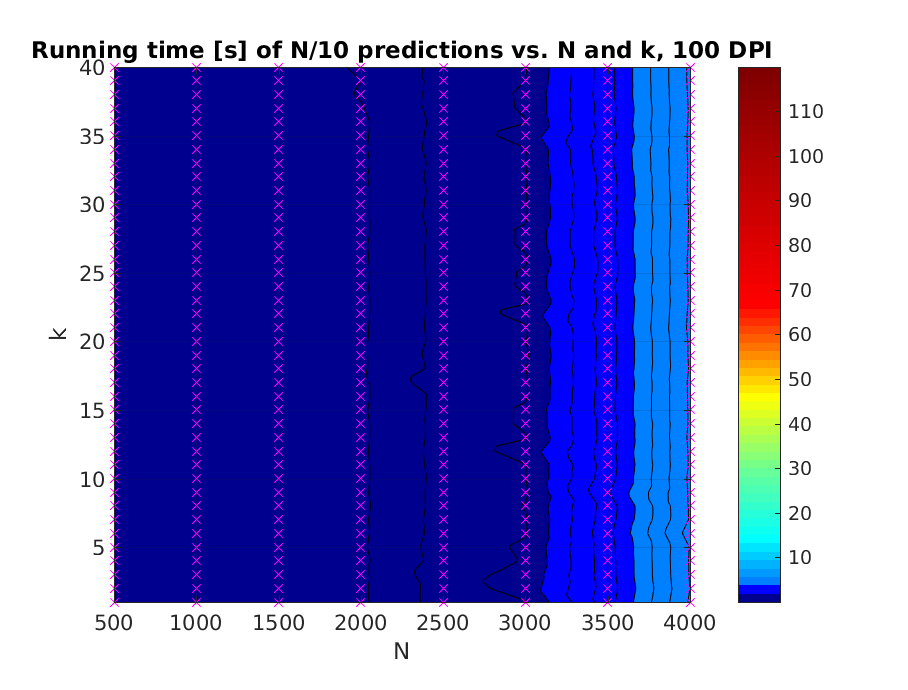
\includegraphics[width = \textwidth]{img/knn-runningTimeVsKVSN-G2M2-dpi100}
		\caption{100 DPI}
	\end{subfigure}
	\begin{subfigure}{0.32\textwidth}
		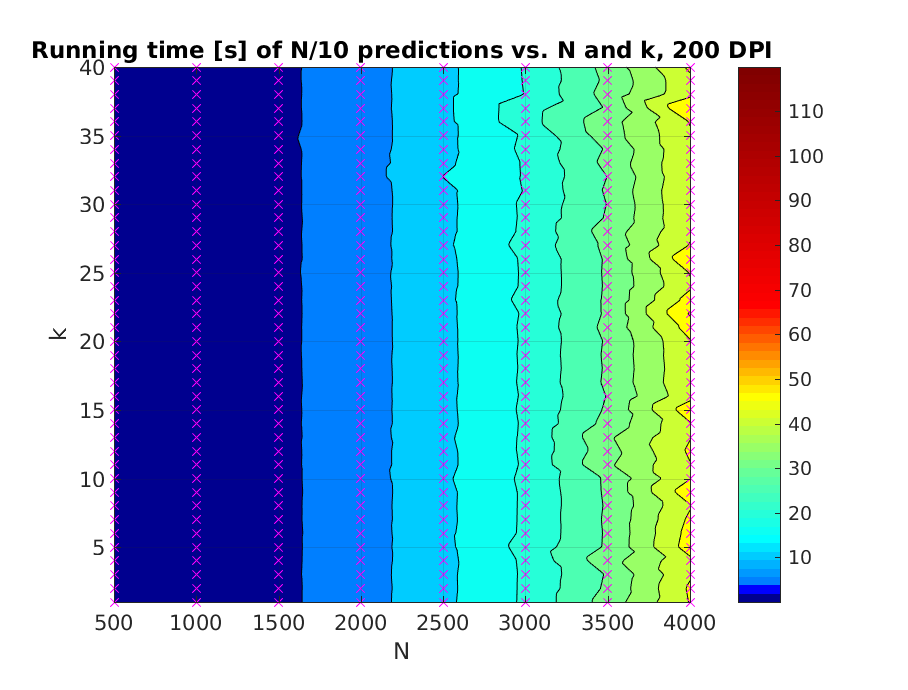
\includegraphics[width = \textwidth]{img/knn-runningTimeVsKVSN-G2M2-dpi200}
		\caption{200 DPI}
	\end{subfigure}
	\begin{subfigure}{0.32\textwidth}
		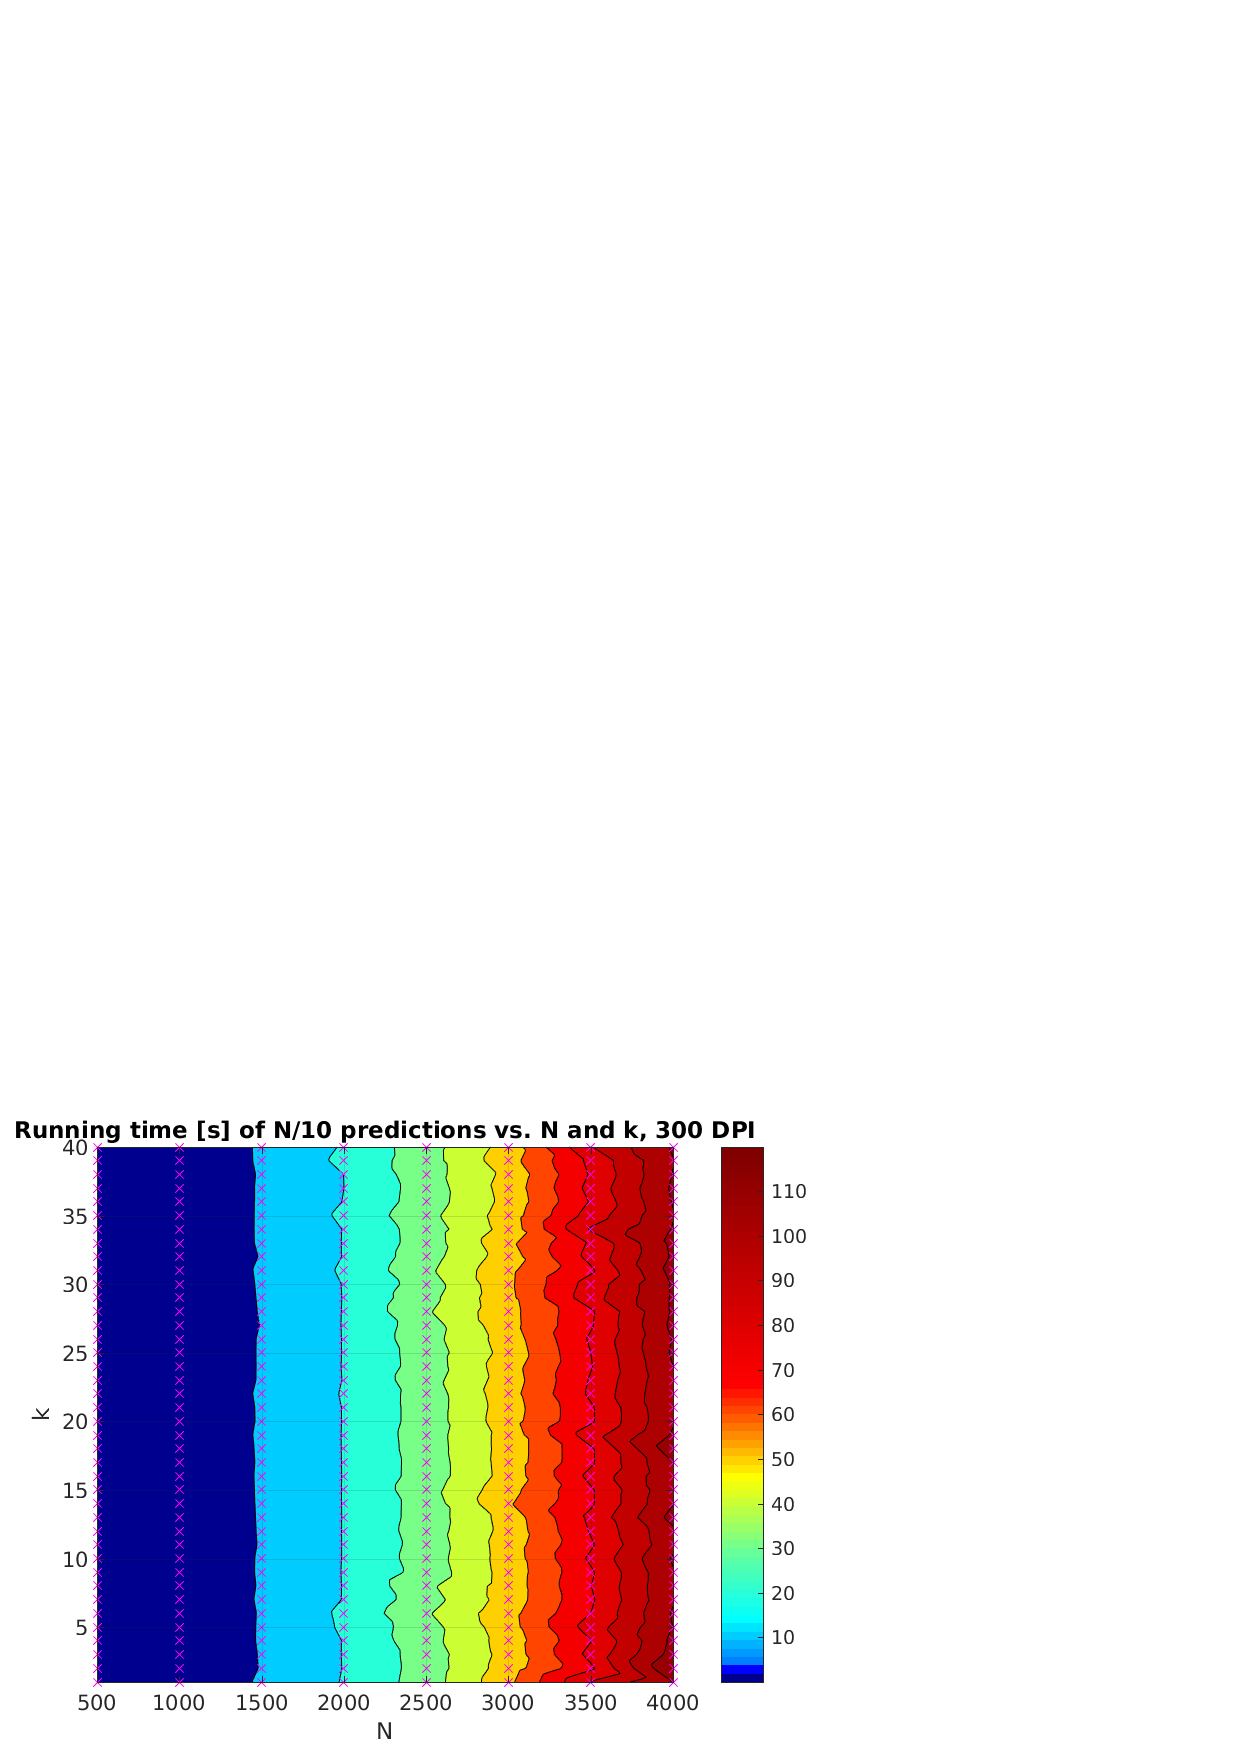
\includegraphics[width = \textwidth]{img/knn-runningTimeVsKVSN-G2M2-dpi300}
		\caption{300 DPI}
	\end{subfigure}
	\caption[
	k-NN prediction running time
			vs. dataset size N and k for G2M2 data at various DPI.
	]{
		k-NN prediction running time in seconds
		vs. dataset size N and k for G2M2 data at various DPI.
		}
	\label{fig:knn-runningtime-vs-n-and-k}
\end{figure}

It is clearly seen that running times are much reduced by downsampling,
and that running times increase substantially with N. It is also seen that
the running times do not vary with k.
Figure \ref{fig:knn-runningtime-vs-n-loglog} visualizes the relationship
between running time and N further.
\begin{figure}[h]
	\centering
	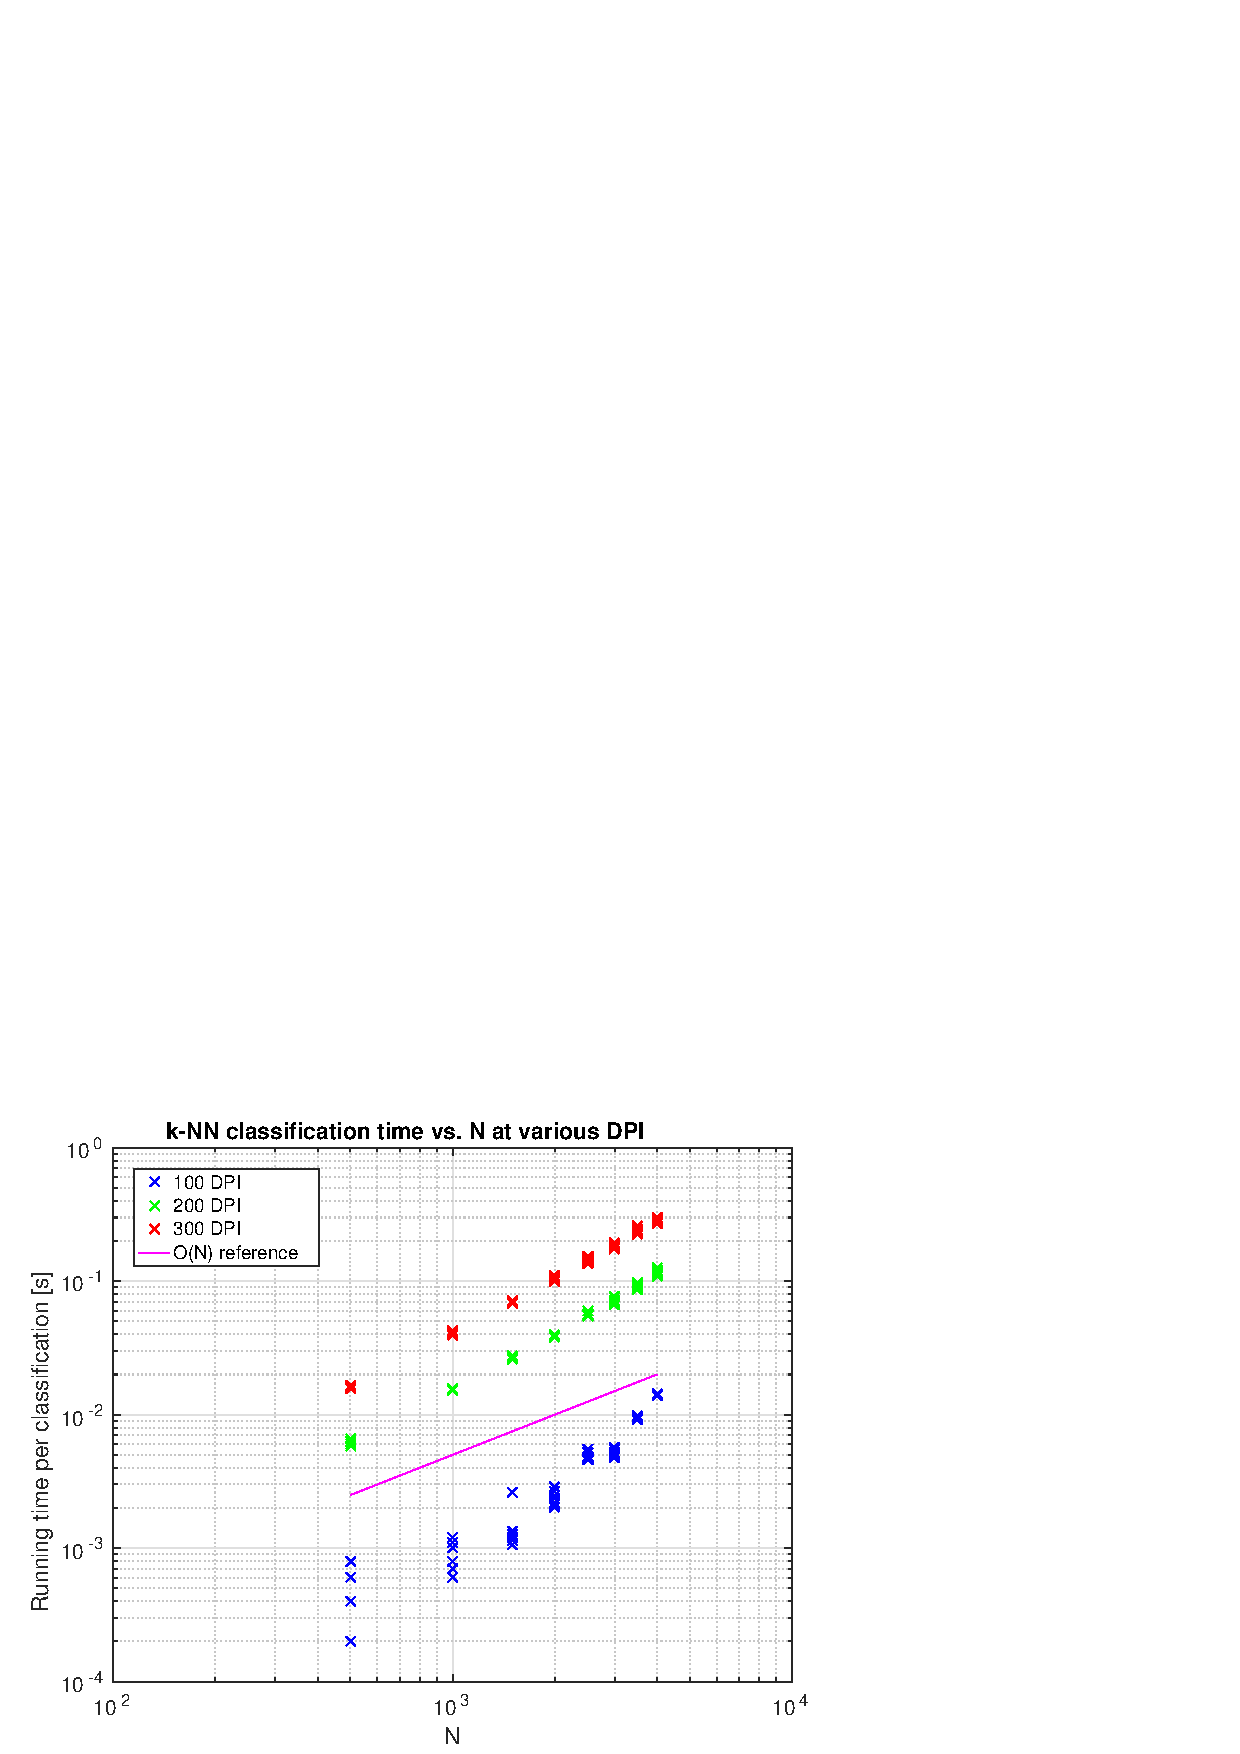
\includegraphics[width = 0.5\textwidth]{img/knn-runningTimeVsNVsDPI-G2M2}
	\caption[log-log plot of k-NN prediction running time vs. N at various DPI.]{
		log-log plot of k-NN prediction running time in seconds vs. N at various DPI.
		\(5\cdot{}10^{-6}\cdot{}N\) reference line also plotted.
	}
	\label{fig:knn-runningtime-vs-n-loglog}
\end{figure}

It can be seen from figure \ref{fig:knn-runningtime-vs-n-loglog} that
the classification time complexity is larger than \(O(N)\).

\subsection{Smoothing}
Figure \ref{fig:knn-AccVsKVsSigma-G2M2},
displays k-NN prediction accuracy vs. smoothing parameter \(\sigma\)
and number of neighbours k on the G2M2 dataset, at various pixel densities.

\begin{figure}[h]
	\centering
	\begin{subfigure}{0.32\textwidth}
		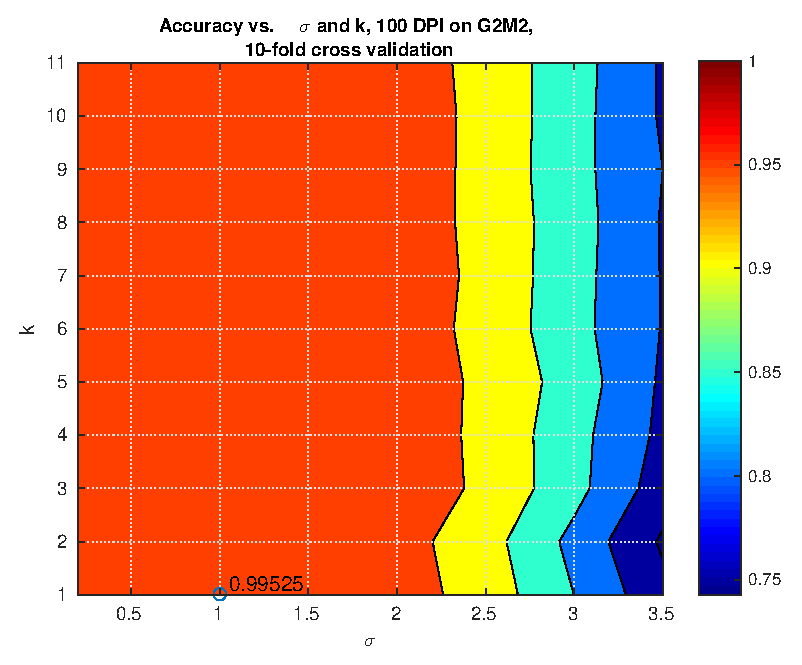
\includegraphics[width = \textwidth]{img/knn-AccVsKVsSigma-G2M2-dpi100-cv10}
		\caption{100 DPI}
	\end{subfigure}
	\begin{subfigure}{0.32\textwidth}
		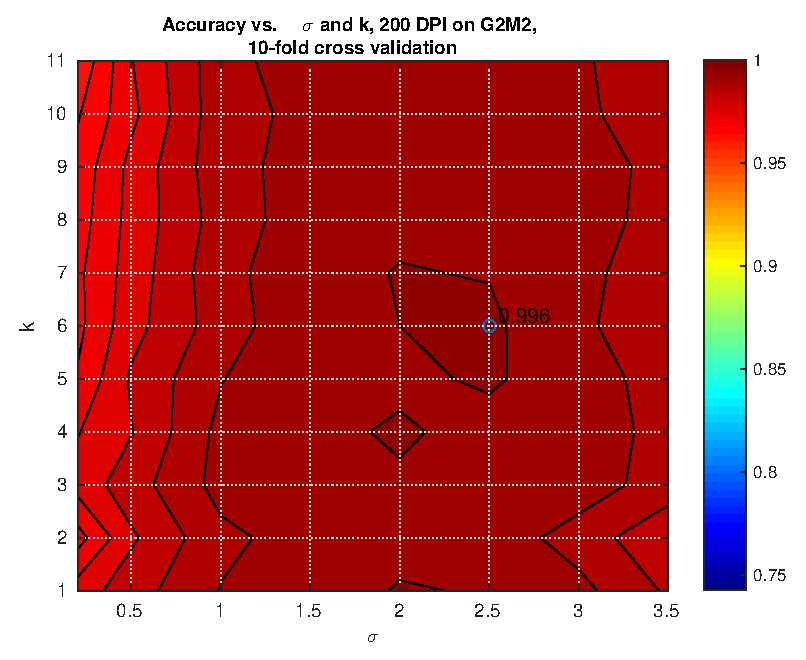
\includegraphics[width = \textwidth]{img/knn-AccVsKVsSigma-G2M2-dpi200-cv10}
		\caption{200 DPI}
	\end{subfigure}
	\begin{subfigure}{0.32\textwidth}
		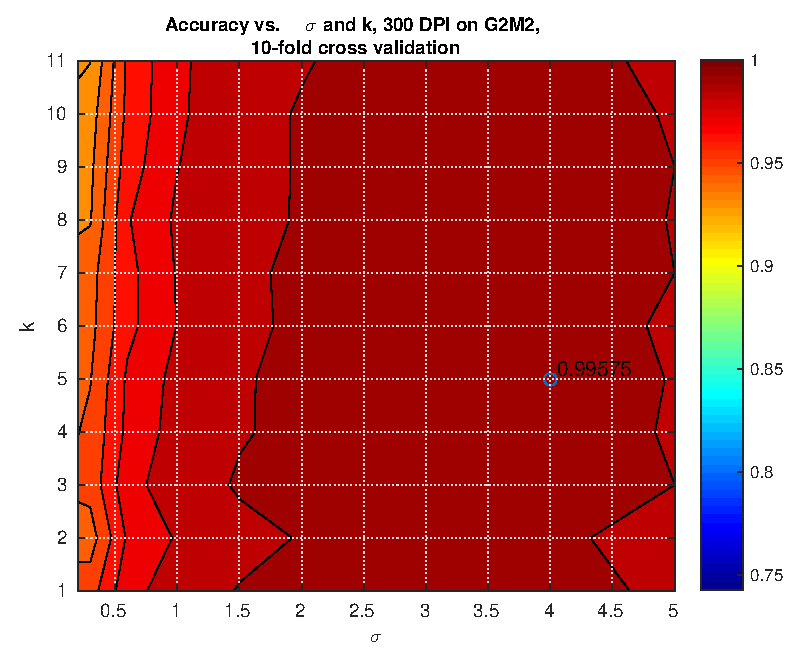
\includegraphics[width = \textwidth]{img/knn-AccVsKVsSigma-G2M2-dpi300-cv10}
		\caption{300 DPI}
	\end{subfigure}
	\caption[k-NN prediction accuracy vs. smoothing parameter $\sigma$
			and k at various DPI.]{
		k-NN prediction accuracy vs. smoothing parameter $\sigma$
		and k for G2M2 data at various DPI.
		}
	\label{fig:knn-AccVsKVsSigma-G2M2}
\end{figure}

\subsection{Principal Component Analysis}
Figure \ref{fig:principal-components} shows the first ten principal
components for all the data, at various DPI.
The normalized intensity \(I_i\) of each pixel in the PC visualization
depends on the weighed contribution \(w_i\) of the pixel position to the principal component
and is determined by
\(I_i=\frac{\left|w_i\right|-\left|w\right|_{min}}{\left|w\right|_{max}-\left|w\right|_{min}}\)
.
\begin{figure}[h]
\centering
\setlength\tabcolsep{1pt}
\begin{tabular}{r*{10}{c}}
Preprocessing & PC1 & PC2 & PC3 & PC4 & PC5 & PC6 & PC7 & PC8 & PC9 & PC10 \\
100 DPI, \(\sigma\)=1
 & 
\includegraphics[width=\smallfigscale]{img/pca-All-dpi100-sigma1-pc1} 
 & 
\includegraphics[width=\smallfigscale]{img/pca-All-dpi100-sigma1-pc2} 
 & 
\includegraphics[width=\smallfigscale]{img/pca-All-dpi100-sigma1-pc3} 
 & 
\includegraphics[width=\smallfigscale]{img/pca-All-dpi100-sigma1-pc4} 
 & 
\includegraphics[width=\smallfigscale]{img/pca-All-dpi100-sigma1-pc5} 
 & 
\includegraphics[width=\smallfigscale]{img/pca-All-dpi100-sigma1-pc6} 
 & 
\includegraphics[width=\smallfigscale]{img/pca-All-dpi100-sigma1-pc7} 
 & 
\includegraphics[width=\smallfigscale]{img/pca-All-dpi100-sigma1-pc8} 
 & 
\includegraphics[width=\smallfigscale]{img/pca-All-dpi100-sigma1-pc9} 
 & 
\includegraphics[width=\smallfigscale]{img/pca-All-dpi100-sigma1-pc10} 
\\
200 DPI, \(\sigma\)=2.5
 & 
\includegraphics[width=\smallfigscale]{{img/pca-All-dpi200-sigma2.5-pc1}.png} 
 & 
\includegraphics[width=\smallfigscale]{{img/pca-All-dpi200-sigma2.5-pc2}.png} 
 & 
\includegraphics[width=\smallfigscale]{{img/pca-All-dpi200-sigma2.5-pc3}.png} 
 & 
\includegraphics[width=\smallfigscale]{{img/pca-All-dpi200-sigma2.5-pc4}.png} 
 & 
\includegraphics[width=\smallfigscale]{{img/pca-All-dpi200-sigma2.5-pc5}.png} 
 & 
\includegraphics[width=\smallfigscale]{{img/pca-All-dpi200-sigma2.5-pc6}.png} 
 & 
\includegraphics[width=\smallfigscale]{{img/pca-All-dpi200-sigma2.5-pc7}.png} 
 & 
\includegraphics[width=\smallfigscale]{{img/pca-All-dpi200-sigma2.5-pc8}.png} 
 & 
\includegraphics[width=\smallfigscale]{{img/pca-All-dpi200-sigma2.5-pc9}.png} 
 & 
\includegraphics[width=\smallfigscale]{{img/pca-All-dpi200-sigma2.5-pc10}.png} 
\\
300 DPI, \(\sigma\)=4
 & 
\includegraphics[width=\smallfigscale]{img/pca-All-dpi300-sigma4-pc1} 
 & 
\includegraphics[width=\smallfigscale]{img/pca-All-dpi300-sigma4-pc2} 
 & 
\includegraphics[width=\smallfigscale]{img/pca-All-dpi300-sigma4-pc3} 
 & 
\includegraphics[width=\smallfigscale]{img/pca-All-dpi300-sigma4-pc4} 
 & 
\includegraphics[width=\smallfigscale]{img/pca-All-dpi300-sigma4-pc5} 
 & 
\includegraphics[width=\smallfigscale]{img/pca-All-dpi300-sigma4-pc6} 
 & 
\includegraphics[width=\smallfigscale]{img/pca-All-dpi300-sigma4-pc7} 
 & 
\includegraphics[width=\smallfigscale]{img/pca-All-dpi300-sigma4-pc8} 
 & \includegraphics[width=\smallfigscale]{img/pca-All-dpi300-sigma4-pc9} 
 & \includegraphics[width=\smallfigscale]{img/pca-All-dpi300-sigma4-pc10} 
\end{tabular}
\caption[Principal components at various DPI.]
{Principal components at various DPI.}
\label{fig:principal-components}
\end{figure}

It is observed that the principal components are very similar
at the three pixel densities, up until principal component 7,
at which point differences are more clearly seen.

Figure \ref{fig:pca-cumvar} shows the cumulated proportion of variance
explained vs. the number of principal components used for data representation,
based on an analysis of all data.
The elbow point is observed at a cumulated variance of approximately 0.95.
\begin{figure}[h]
\centering
\includegraphics[width=\figscale]{img/pca-All-cumvar-dpi100-sigma1}
\caption[Cumulated variance explained by PCA]
{Cumulated proportion of variance explained vs. number of principal components.
All data was used for the analysis, preprocessed with DPI=100 and \(\sigma=1\).}
\label{fig:pca-cumvar}
\end{figure}

\subsection{Parameter optimization}
Figure \ref{fig:pca-knn-acc-vs-k} shows k-NN classification
accuracy vs. number of neighbours k on the \(D_{FEWER}\) dataset.
It is observed that the accuracy is maximal with k=5.
\begin{figure}[h]
\centering
\includegraphics[width=\figscale]{img/pca-knn-acc-vs-k-dpi100-sigma1}
\caption[k-NN classification accuracy vs. k on $D_{FEWER}$, \textbf{LOO}.]
{
k-NN classification accuracy vs. k on $D_{FEWER}$, \textbf{LOO}, DPI=100, $\sigma=1$.
}
\label{fig:pca-knn-acc-vs-k}
\end{figure}

Figure \ref{fig:pca-svm-acc-vs-C} shows SVM classification accuracy vs.
cost of constraints violation C on the \(D_{FEWER}\) dataset.
It is observed that the accuracy does not vary significantly with C.
However, the maximal mean overall accuracy was found at C=0.5.
\begin{figure}[h]
\centering
\includegraphics[width=\figscale]{img/pca-svm-acc-vs-C-dpi100-sigma1}
\caption[SVM classification accuracy vs. C on $D_{FEWER}$, \textbf{LOO}.]{
SVM classification accuracy vs. C on $D_{FEWER}$, \textbf{LOO}, DPI=100, $\sigma=1$.
The SVM kernel is polynomial with degree 2 and scale 0.1.
}
\label{fig:pca-svm-acc-vs-C}
\end{figure}

\subsection{Quality of individual datasets for classification}
Figure \ref{fig:singlePersonIndividual} shows k-NN and SVM
classification accuracy when applied to each persons dataset separately.
It is observed that the k-NN classification accuracy is lower than the SVM
classification accuracy on most of the datasets.
It is also observed that the lowest accuracy is found with data from \(G2M1\).
\begin{figure}[h]
\centering
\includegraphics[width=\figscale]{img/singlePersonIndividual-dpi100-sigma1}
\caption[Classification accuracy on individual datasets.]{
k-NN and SVM classification accuracy on each persons dataset, based on 10-fold cross validation.
}
\label{fig:singlePersonIndividual}
\end{figure}

\subsection{Comparison of classification algorithms}
k-NN and SVM classification accuracies are shown for three different
classification problems in figure \ref{fig:knn-vs-svm-full},
and a zoomed view is seen in figure \ref{fig:knn-vs-svm-zoomed}.
\begin{figure}[h]
\centering
\begin{subfigure}{\figscale}
\centering
\includegraphics[width=\figscale]{img/knn-vs-svm-full-dpi100-sigma1}
\caption[k-NN and SVM classification accuracies, full view.]
{Full view.}
\label{fig:knn-vs-svm-full}
\end{subfigure}
\\
\vspace{0.5cm}
\begin{subfigure}{\figscale}
\centering
\includegraphics[width=\figscale]{img/knn-vs-svm-zoomed-dpi100-sigma1}
\caption[k-NN and SVM classification accuracies, zoomed view.]
{
Zoomed view.
}
\label{fig:knn-vs-svm-zoomed}
\end{subfigure}
\caption[k-NN and SVM classification accuracies]{
"Single persons" is the mean accuracy of the overall accuracy of 10-fold cross validation run for each individual.
"All mixed" is the mean accuracy based on $D_{ALL}$, \textbf{MIX}.
"All LOO" is the mean accuracy based on $D_{ALL}$, \textbf{LOO}.
The k-NN classifier was trained with k=5. The SVM classifier was trained with degree=2, scale=0.1 and C=0.5.
}
\end{figure}

For the "Single persons" problem, the SVM classifier has the highest mean accuracy.
For the "All mixed" problem, the k-NN classifier has the highest mean accuracy.
For the "All LOO" problem, the SVM classifier has the highest mean accuracy.

The significance of these three results was tested by subtracting the classification
accuracies of the two algorithms from each other,
and applying a Z-test with a null hypothesis of zero mean.
With a level of significance \(\alpha=0.05\),
only the difference in the "All mixed" problem is significant.
The p-values of the three Z-tests are listed in table \ref{tb:ztest}.
\begin{table}[h]
\centering
\caption[Z-test results]
{
Z-test results for the null hypotheses that k-NN accuracy has
the same mean as the SVM accuracy, \(H_0:\mu\left(\text{k-NN}\right)-\mu\left(\text{SVM}\right)=0\), for three different classification problems.
}
\begin{tabular}{|r||c|c|c|}
\hline
 & Single persons & All mixed & All LOO
 \\
 \hline
p-value & 0.28 & 0.0025 & 0.087
\\
CI (difference in accuracy)& \(\left[-0.022;0.0064\right]\)
& \(\left[0.0034;0.016\right]\)
& \(\left[-0.11;0.0072\right]\)
\\
\(H_0\) rejected & No & Yes & No
\\
\hline
\end{tabular}
\label{tb:ztest}
\end{table}
%H=0 indicates that the null hypothesis ("mean is M")
%cannot be rejected at the 5% significance level.  H=1
%indicates that the null hypothesis can be rejected at the 5% level.
%spH =
%     0
%spP =
%   0.276940767397244
%spCI =
%  -0.022269551784590
%   0.006378247436764
%amH =
%     1
%amP =
%   0.002458171781170
%amCI =
%   0.003382419250751
%   0.015791493792727
%alH =
%     0
%alP =
%   0.086657366992428
%alCI =
%  -0.107175202166838
%   0.007196941297274

Figure \ref{fig:prediction-times} shows the prediction times per digit
of the k-NN and SVM classifiers, when trained with \(D_{ALL}\).
These prediction times were obtained by repeating the prediction
of all \(G2M2\) digits 30 times, taking the average and dividing by the number
of digits (4000).
It is observed from figure \ref{fig:prediction-times} that
the SVM classifier is more than twice as fast as the k-NN classifier,
when each is trained with \(D_{ALL}\).
\begin{figure}[h]
\centering
\includegraphics[width=\figscale]{img/prediction-times}
\caption[Prediction times per digit]
{
Prediction times per digit. Each classifier was trained with \(D_{ALL}\)
and applied to all \(G2M2\) digits 30 times.
The shown results are the average prediction times per digit.
}
\label{fig:prediction-times}
\end{figure}
%4000 digits:
%"knn_time_mean","knn_time_sdev","svm_time_mean","svm_time_sdev"
%32.4009333333333,4.32796005888043,10.4381333333333,1.58063548401692 %Result
				   %And
\section{Discussion}%Discussion
\section{Conclusions}
\label{sec:conclusion}
%The main purpose of this project is to compare two classification algorithms,
%k-Nearest Neighbours (k-NN) and Support Vector Machines (SVM),
%for handwritten digit recognition.
%The second purpose of this project is to achieve good classification performance,
%and thus, some preprocessing is needed.
%Lastly, as the digits used in this project
%were written by a class of 23 always competitive students,
%it was chosen to estimate the quality of the hand written digits
%and identify the student with the worst hand writing.
%This required a definition of hand written digit quality,
%which is also presented here.
k-NN with number of neighbours k=5 achieves significantly higher overall 
classification accuracy than SVM with polynomial kernel of degree 2
with scale factor 0.1 and cost of constraints violation C=0.5,
with \(\alpha=0.05\),
when each algorithm is trained with a dataset of hand written digits
from a class of 23 people, and tested on a dataset
with digits written by the same people.
When the training set only contains data from 22 people,
and the test set is written by a person not in the training
set, k-NN does not perform significantly worse
than SVM, although a lower overall accuracy was observed.
Neither does the k-NN classifier perform significantly worse than SVM
when applied to one persons data at a time,
although a lower overall accuracy was observed.

The highest obtained overall classification accuracy is 0.854 with a standard
deviation of 0.0205, for the SVM classifier.

A successful preprocessing scheme involving the perspective transform,
gaussian blur and Principal Component Analysis was implemented.

Person \(G2M1\) (one of the authors) has the worst digit hand writing of the 2016 SML class,
when the writing quality is measured by classification
error on own data. This means \(G2M1\) has the least
within-digit consistent and between-digit varied
hand writing.


\newpage
%\bibliographystyle{ieeetr}
\bibliography{bibliography}
\end{document}

